\documentclass[border=10pt]{standalone}

\usepackage{tikz}
\usepackage{tikzsymbols}
\usetikzlibrary{calc,patterns,shapes.geometric}

\def\centerarc[#1](#2)(#3:#4:#5){\draw[#1] ($(#2)+({#5*cos(#3)},{#5*sin(#3)})$) arc (#3:#4:#5);}

\begin{document}
	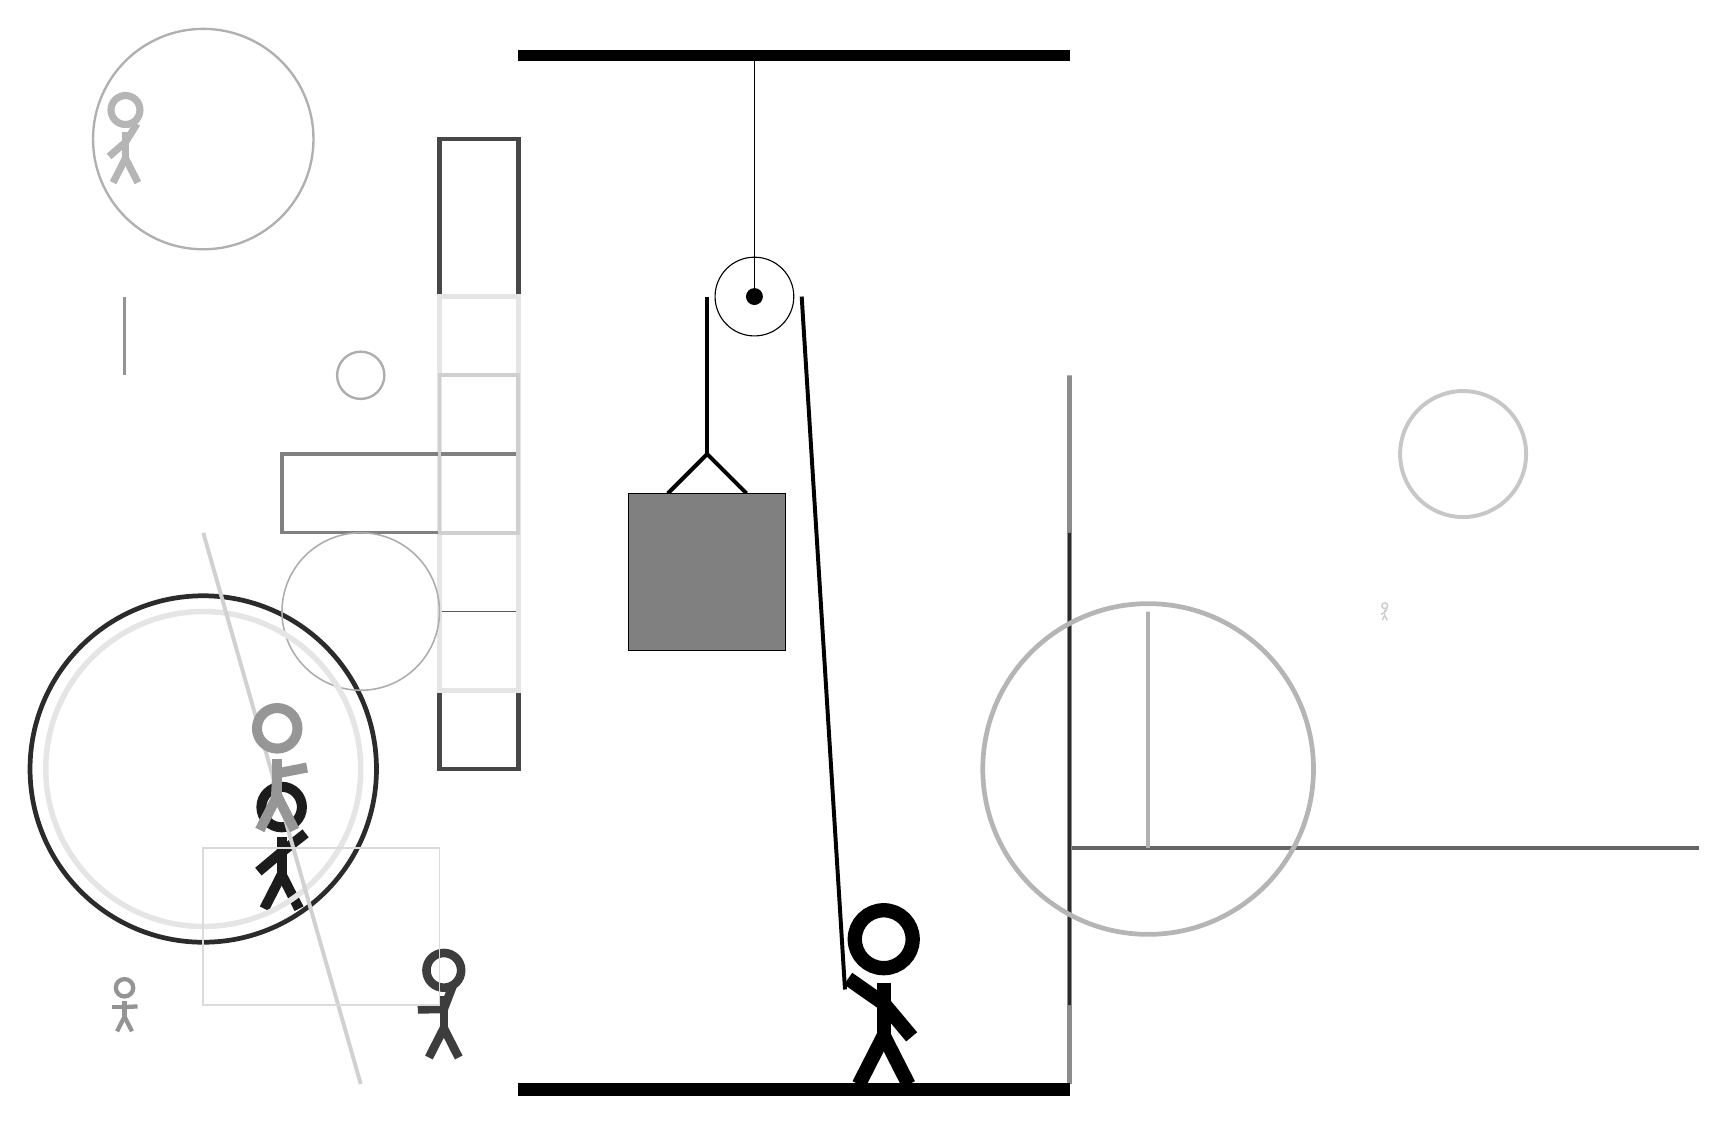
\begin{tikzpicture}
		%%%%% START %%%%%
		
		\draw[fill=black] (-2, 10) rectangle (5, 10.125);
		
		\draw (1, 7) circle (0.5);
		\draw[fill=black] (1, 7) circle (0.1);
		\draw (1, 10) -- (1, 7);
		
		\node[line width=0.3mm, color=black!89] at (-5, 0) {\Strichmaxerl[7][40][38]};
		
		\draw[line width=0.6mm, color=black!72] (-2, 9) rectangle (-3, 1);
		\node[line width=0.3mm, color=black!76] at (-3, -2) {\Strichmaxerl[6][1][69]};
		\draw[line width=0.5mm, color=black!60](5, 0) -- (13, 0);
		
		\draw[line width=0.7mm, color=black!45] (5, 6) rectangle (5, -3);
		\draw[line width=0.2mm, color=black!65] (-3, 2) rectangle (-2, 3);
		\draw [line width=0.3mm, color=black!32](-4, 6) circle (0.3);
		\draw[line width=0.3mm, color=black!83] (5, 4) rectangle (5, -2);
		\node[line width=0.2mm, color=black!29] at (-7, 9) {\Strichmaxerl[5][41][58]};
		\draw[line width=0.6mm, color=black!10] (-3, 7) rectangle (-2, 2);
		\draw [line width=0.6mm, color=black!83](-6, 1) circle (2.2);
		\node[line width=0.2mm, color=black!20] at (9, 3) {\Strichmaxerl[1][33][57]};
		\draw[line width=0.5mm, color=black!42](-7, 7) -- (-7, 6);
		
		\draw[line width=0.4mm, color=black!50] (-2, 5) rectangle (-5, 4);
		\draw [line width=0.2mm, color=black!32](-4, 3) circle (1.0);
		\node[line width=0.6mm, color=black!42] at (-7, -2) {\Strichmaxerl[3][0][3]};
		
		\draw [line width=0.7mm, color=black!10](-6, 1) circle (2.0);
		\draw [line width=0.7mm, color=black!70](-4, 7) circle (0.0);
		\draw[line width=0.5mm, color=black!19] (-3, 6) rectangle (-2, 4);
		
		\draw [line width=0.6mm, color=black!29](6, 1) circle (2.1);
		\draw[line width=0.5mm, color=black!18](-4, -3) -- (-6, 4);
		
		\draw[line width=0.2mm, color=black!14] (-3, -2) rectangle (-6, 0);
		\draw [line width=0.3mm, color=black!31](-6, 9) circle (1.4);
		\draw [line width=0.5mm, color=black!22](10, 5) circle (0.8);
		\draw[line width=0.5mm, color=black!30] (6, 0) rectangle (6, 3);
		
		\node[line width=0.3mm, color=black!41] at (-5, 1) {\Strichmaxerl[7][87][11]};
		
		\draw[line width=0.5mm] (-0.1, 4.5) -- (0.4, 5.0) -- (0.9, 4.5);
		\draw[fill=black!50] (-0.6, 4.5) rectangle (1.4, 2.5);
		
		\draw[line width=0.5mm] (0.4, 7) -- (0.4, 5.0);
		\centerarc[line width=0.5mm](1, 7)(0:180:0.6);
		\draw[line width=0.5mm](1.6, 7) -- (2.15, -1.8);
		
		\node at (2.6, -1.9) {\Strichmaxerl[10][-35][-50]};
		
		\draw[fill=black] (-2, -3) rectangle (5, -3.15);
		
		%%%%% END %%%%%
	\end{tikzpicture}
\end{document}